\documentclass[border=4mm]{standalone}
\usepackage{fontspec}
\setmainfont{Latin Modern Sans}
\usepackage{tikz}
\usetikzlibrary{arrows.meta,positioning}
\begin{document}
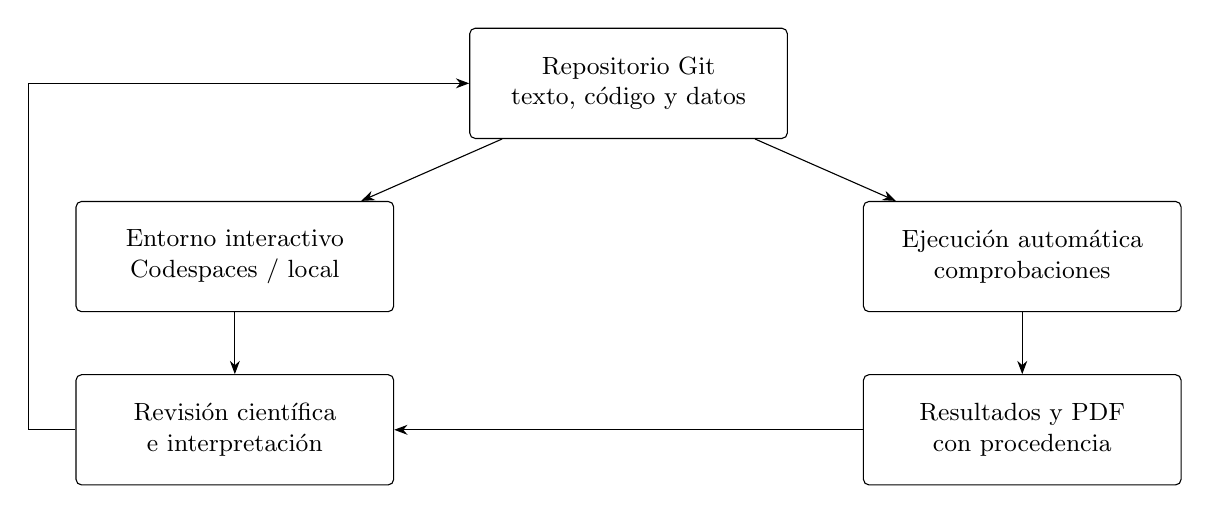
\begin{tikzpicture}[>=Stealth,box/.style={draw,rounded corners=2pt,align=center,text width=38mm,minimum height=14mm,font=\small},every edge/.style={draw,->}]

\node[box] (source) at (5,0) {Repositorio Git\\texto, código y datos};
\node[box] (edit) at (0,-2.2) {Entorno interactivo\\Codespaces / local};
\node[box] (ci) at (10,-2.2) {Ejecución automática\\comprobaciones};
\node[box] (review) at (0,-4.4) {Revisión científica\\e interpretación};
\node[box] (pdf) at (10,-4.4) {Resultados y PDF\\con procedencia};
\path (source) edge (edit) (source) edge (ci) (edit) edge (review) (ci) edge (pdf) (pdf) edge (review);
\draw[->] (review.west) -- ++(-0.6,0) |- (source.west);
\end{tikzpicture}
\end{document}
